% ---------------------------------------------------------------------------
% Version history (visible on page 1 and in the PDF metadata; one line per
% content revision, newest first).  The version counts content revisions; the
% build time on page 1 is generated at compile time (\buildstamp), so it always
% matches the file it is printed on.
%   v1.3 2026-11-17  a correction to v1.2: the share of bytes was wrong.
%                     "45 % of int8's bytes" is the saving, not the share.  The
%                     measured share is 54.5 % (144 against 264 bytes per cell
%                     and head; the record computes it at
%                     bench/results/2026-11-14-q4u32-fastpath/README.md:503).
%                     The abstract, the quoted log line and every place that
%                     states the share are corrected; no other number changes.
%   v1.2 2026-11-17  a correction to v1.1, from reading the kernel: the
%                     statement that a 64-value block "spans two kernel groups
%                     and cannot apply its one scale per group" was wrong.
%                     The step of a 64-value block is constant inside each
%                     32-dimension group, so the kernel serves it with the
%                     same fold it uses now; what the change costs is the
%                     block index, the lane's offset and a four-quadrant
%                     nibble rule --- three local changes, not a blocker.
%                     A 16-value block, on the other hand, is the one that
%                     cannot be served (two blocks inside one group, one step
%                     per group).  The trade is therefore a trade and not a
%                     closure: 0.25 bit per value (about 1.2 % more resident
%                     experts on the measured card) against 0.92 dB.  The
%                     abstract and Section 6.3 are corrected; the group size
%                     stays at 32, for a stated reason.
%   v1.1 2026-11-17  the last open knob of the format is closed (A.27): the
%                     block's group size.  A group of 16 wins 1.19 dB and
%                     costs 0.5 bit per value more, a group of 64 loses
%                     0.92 dB and saves 0.25 bit per value; neither is
%                     buildable, because the prompt attention applies the
%                     scale per group of 32 dimensions and a block is a row
%                     along the head dimension.  The format is therefore
%                     fixed at 4.5 bit per cell, one step per 32 values, a
%                     uniform grid, no codebook, no zero point, no
%                     calibration; the ablation table gains the two rows
%                     and the abstract states the closure.
%   v1.0 2026-11-17  the first version of the q4u32 paper.  It reports the
%                     product path that the engine series A.16-A.23 measured:
%                     a 4-bit KV pool that the RDNA4 prompt kernel reads
%                     directly (the matrix core), the format it needs (a
%                     uniform grid with a fitted step per 32-value block, no
%                     codebook, no per-model table), the ablation that says
%                     which parts of it are load-bearing (the per-block scale
%                     is; the codebook is not: 0.43 dB), the closed channel
%                     axis (A.26: a per-coordinate scale is 1.26 dB WORSE on
%                     the key side, in 12 of 12 layers), and the product
%                     decision (the card chooses the format on gfx12; every
%                     other card and every upstream engine keeps 8-bit).
%                     The RDNA3 and APU arms are pre-registered and open
%                     (A.24, A.25): the hardware is not here.
% ---------------------------------------------------------------------------
\documentclass[10pt,twocolumn]{article}
\usepackage[T1]{fontenc}
% Page geometry: ACM sigplan (10pt conference) --- US Letter, 1in top/bottom,
% 0.75in side margins, 2pc column separation.
\usepackage[letterpaper,top=1in,bottom=1in,margin=0.75in,columnsep=2pc,heightrounded]{geometry}
% Fonts: the ACM template pair --- Linux Libertine (text) and Inconsolata (mono).
\usepackage[tt=false]{libertine}
\usepackage{libertinust1math}
\usepackage[varqu]{zi4}
\usepackage{microtype}
\usepackage{booktabs}
\usepackage{array}
\usepackage{tabularx}
\usepackage{xcolor}
\usepackage{hyperref}
\usepackage{amsmath}
\usepackage{enumitem}
\usepackage{multirow}
\usepackage{titlesec}
\usepackage{caption}
\usepackage{tikz}

% ACM sigplan heading styles: bold \Large sections, bold normal-size subsections,
% ragged-right, tight spacing.
\titleformat{\section}{\Large\bfseries\raggedright}{\thesection}{0.7em}{}
\titleformat{\subsection}{\normalsize\bfseries\raggedright}{\thesubsection}{0.6em}{}
\titleformat{\subsubsection}{\normalsize\bfseries\raggedright}{\thesubsubsection}{0.5em}{}
\titlespacing*{\section}{0pt}{1.2ex plus .2ex minus .2ex}{0.55ex plus .1ex}
\titlespacing*{\subsection}{0pt}{1.0ex plus .2ex minus .2ex}{0.45ex plus .1ex}
\titlespacing*{\subsubsection}{0pt}{0.9ex plus .2ex minus .2ex}{0.4ex plus .1ex}

% ACM caption style: bold label, small text.
\captionsetup{labelfont=bf,font=small,skip=6pt}

% Build stamp: taken from the compile-time clock (the same \year/\month/\day/\time
% pdfTeX writes into the PDF's /CreationDate), so the visible version line cannot
% drift from the file it is printed on.  Zero-padded by hand because the engine's
% numbers are not.
% \numexpr rounds a division, so \time/60 is not the hour (634/60 gives 11,
% not 10).  Count registers truncate, and computing the two values once in the
% preamble keeps \buildstamp fully expandable for the PDF metadata.
\newcount\bsthour
\newcount\bstminute
\bsthour=\time \divide\bsthour by 60
\bstminute=\bsthour \multiply\bstminute by 60
\bstminute=-\bstminute \advance\bstminute by \time
\newcommand{\twod}[1]{\ifnum#1<10 0\fi\number#1}
\newcommand{\buildstamp}{\number\year-\twod{\month}-\twod{\day}, \twod{\bsthour}:\twod{\bstminute} CET}

% ACM link colors.
\definecolor{ACMPurple}{cmyk}{0.55,1,0,0.15}
\definecolor{ACMDarkBlue}{cmyk}{1,0.58,0,0.21}
\hypersetup{colorlinks,linkcolor=ACMPurple,citecolor=ACMPurple,urlcolor=ACMDarkBlue,
  pdftitle={q4u32: A 4-bit KV Cache the Matrix Core Can Read},
  pdfauthor={Matthias Kronenberger},
  pdfsubject={Version 1.3, built \buildstamp; first version 2026-11-17}}

\setlength{\parindent}{10pt}

\begin{document}

% Full-width ACM conference title block, then the two columns start with the abstract.
\twocolumn[{%
  \begin{center}
    {\LARGE\bfseries q4u32: A 4-Bit KV Cache the Matrix Core Can Read\par}
    \vspace{0.6em}
    {\large The prompt path of RDNA4 reading the 4-bit KV pool directly, and what the format needs to be the default\par}
    \vspace{1.0em}
    {\large Matthias Kronenberger\par}
    \vspace{0.35em}
    {\small Version 1.3 \,\textperiodcentered\, built \buildstamp\ \,\textperiodcentered\, first version 2026-11-17\par}
  \end{center}
  \vspace{1.0em}
}]

\noindent\textbf{Abstract}\par
\vspace{0.6ex}
\noindent
On RDNA4 the prompt (prefill) of a transformer runs on the matrix cores, and the attention kernel reads the
key/value cache there. A 4-bit KV cache could not be read by that kernel, so it ran on the decode kernel
instead --- 2.5 times slower, which turned the memory win into a loss. This paper reports the format that
removes that loss. The format is \texttt{q4u32}: after the same Walsh--Hadamard rotation the cache already
uses, a uniform grid on blocks of 32 values with a least-squares-fitted step per block, 4.5 bit per cell
against \texttt{int8}'s 8.25. Its property is that it is \emph{affine along the head dimension}, which is
exactly the map the batched prompt attention already applies per group of 32 dimensions: the operand becomes
$(\text{code}-8)\cdot d$, no table, no codebook, no per-model artifact. We measure the implementation on a
Windows RDNA4 box (gfx1201): the parity harness is green (worst deviation $5.7\cdot10^{-6}$ against an FP64
reference on a scale of $\approx 7.5$, the same order as the decode kernel), the engine's own route line
appears in every run, and the prompt rate is level with \texttt{int8} ($-1.8\%$ mean, $-2.1\%$ median over
nine and six requests at 32K) while the cache carries 54.5\,\% of the bytes --- which the expert cache takes up
as \textbf{+18.7\%} more resident slots. Without the matrix path the same format is 2.5 times slower, so the
path is not an optimization of the format but its precondition. The ablation says what the format needs:
the per-block scale is load-bearing (a fitted Lloyd codebook on the same blocks costs 0.43\,dB; a
power-of-two step costs 1.81\,dB), the codebook is not (the ``codebook barely matters'' finding of
UltraQuant, measured here on 1.57 million of our own blocks), and the per-channel axis of the 4-bit
literature is closed: a scale per coordinate instead of per token is \textbf{1.26\,dB worse} on the key side
in 12 of 12 layers, because after the rotation the dynamic range lives in the token, not in the channel.
The block's group size is settled with it (a group of 16 wins 1.19\,dB for half a bit per value more and
cannot be served by the kernel's 32-dimension group at all; a group of 64 loses 0.92\,dB for a quarter of a
bit less and could be served, for about 1.2\,\% more resident experts --- the wrong direction for a format
whose margin over \texttt{int8} is what it was chosen for), so the format is fixed: \textbf{4.5 bit per
cell, one step per 32 values, a uniform grid, no codebook, no zero point, no calibration}. The
product decision follows the measurement and is stated as such: on gfx12 the engine chooses the format, the
Terminal follows it, every other card and every upstream engine keeps 8-bit, and an update never switches
the variant of Strata that is installed.
\par\medskip

\section{Introduction}

A 4-bit key/value cache is the cheapest thing a long-context server can do: it halves the memory that
competes with the expert weights, and on a card whose experts are streamed from the SSD every freed
megabyte is a resident expert. On AMD's RDNA4 the prompt path of the engine runs on the matrix cores, and
the batched prompt attention reads the cache there. That kernel could not read a 4-bit pool: it read
\texttt{int8} codes and reconstructed them, and a 4-bit pool --- which stores a scale next to the codes ---
had to be served by the decode kernel instead. The consequence was measured and it is not subtle: the same
model, the same prompt, the same cache bytes, \textbf{2.5 times slower} (\,\texttt{q4u32} at 264.3 tokens per
second against \texttt{int8} at 663.6 on a 32K needle run). A format that saves 55\% of the cache and costs
60\% of the prompt rate is not a memory optimization; it is a rollback.

This paper reports the format that removes that loss, and the measurements that made it the default.
The format is \texttt{q4u32}: a uniform grid on blocks of 32 values with a fitted step per block, written
after the same Hadamard rotation the cache already applies. It is not a new idea --- the sibling paper's
campaign measured the grid's geometry on this engine's own blocks\,\cite{shear} and found that the uniform
grid with a fitted step is 0.86\,dB \emph{better} than the fitted Lloyd codebook it would replace, and that
the codebook's own cost is 0.43\,dB\,\cite{shear}. What is new here is that the format is read by the
matrix core, that the reading is measured end to end, and that the consequence was taken all the way to
the product: the engine's own default on the cards where the path was measured, and a marking that keeps
an update from replacing it.

Three things make the format fit the kernel, and it is worth separating them, because they are often
confused. First, the prompt attention applies the block scale \emph{per group of 32 dimensions, after that
group's partial sum}; a format whose map along the head dimension is affine therefore rides the kernel for
free. Second, the kernel's hardcoded part is the \emph{value mapping} $(\text{code}-8)$, so a uniform grid
with a fitted step needs no table in the operand, while a codebook format would need one. Third, the
writer must not need anything the kernel cannot reconstruct: \texttt{q4u32} stores a step and the codes,
nothing else. What the format does \emph{not} do is shrink below 4.5 bit per cell: the scale is half a bit
per cell at a group of 32, and that half bit is the price of the group's own dynamic range.

The contributions are: (i) the format and the writer, (ii) the kernel work that reads it --- the 4-bit
pool in the batched prompt attention and the exact-cell window that the sibling paper's format needs,
(iii) the measurements: parity against an FP64 reference, the engine's own route, the prompt rate against
\texttt{int8}, and the expert-cache slots the freed memory buys, (iv) an ablation on the engine's own blocks
that says which parts of the format are load-bearing and closes the channel axis that the 4-bit literature
proposes, and (v) the product rule that follows: the card chooses the format where the path was measured,
everywhere else the last release's behaviour is unchanged.

\paragraph{What this paper is not.} It is not a claim about 4-bit caches in general. The quality of a 4-bit
cache is the sibling paper's subject\,\cite{shear}, and this paper takes the format it selected as given
and asks whether the hardware can serve it. The RDNA3 (gfx11) and the integrated-APU arms are
pre-registered and open (Section~\ref{sec:limits}): the hardware is not on this machine. Every number below
is labelled as a measurement, a citation, a calculation or static analysis; where a number is not a
measurement of this engine, it says so.

\section{The Problem: a cache the prompt kernel cannot read}
\label{sec:problem}

\subsection{The price, measured}

The engine stores the key and the value rows of 12 cache-carrying attention layers of a 48-layer model. Two
formats were compared on the same 32K needle run, the same model, the same machine and the same build
(A.~21, Table~\ref{tab:price}): the 8-bit cache the engine reads natively in the prompt kernel, and a
4-bit cache with a per-block scale. The 4-bit cache was 2.5 times slower --- 264.3 tokens per second
against 663.6 --- because it could not be served by the matrix-core path and fell back to the decode kernel.
The same run, with the routing switch flipped, is what makes the price attributable to the route rather
than to the codec: with the switch off, the 4-bit pool is at 264.3 tokens per second, with it on, it is at
the level of \texttt{int8} (Section~\ref{sec:meas}).

\begin{table}[t]
\centering
\caption{The price of a 4-bit pool without the matrix path (measurement, A.~21: 32K needle run, three
requests, same model, same build, same machine; the level is the slow one, the median over the requests).}
\label{tab:price}
\begin{tabular}{lrr}
\toprule
KV format & prompt rate (tok/s) & route \\
\midrule
\texttt{int8}                & 663.6 & matrix core \\
\texttt{q4u32}, path off     & 264.3 & decode kernel \\
\texttt{q4u32}, path on      & 651.6 & matrix core \\
\bottomrule
\end{tabular}
\end{table}

\subsection{What the prompt kernel does}
\label{sec:kernel}

The batched prompt attention of the engine computes, for a tile of 16 query rows against a tile of 16 key
positions, a matrix product per 32-dimension group and applies the group's scale after the group's partial
sum. Two properties of that kernel decide which formats it can serve, and both are properties of the
\emph{code}, not of the hardware.

\paragraph{The map along the head dimension must be affine.} The scale is applied per group of 32
dimensions, after that group's partial sum. A format whose reconstruction is
$(\text{code}-8)\cdot d$ --- an affine map that may vary along the head dimension --- is therefore served
exactly. A format with a level table ($\text{value}=\text{level}[\text{code}]\cdot d$) is not: the table
would have to be looked up in the operand, once per element. The sibling paper measured that price on this
engine's blocks: the level table costs 0.43\,dB against the uniform grid\,\cite{shear}, and the sibling
campaign's end-to-end run put it at $2.25\times$ the prompt read time of the uniform arm\,\cite{shear}. The
uniform grid is not a compromise here; it is the format the kernel can read without work.

\paragraph{The value mapping is hardcoded.} What the kernel cannot do is a value mapping that is not
$(\text{code}-8)$. That is a one-line constraint on the format, and it is what rules the codebook out of
the fast path. It also rules out a per-block zero point in the fast path (the reconstruction would gain a
per-block constant), which is why the zero point costs half a bit per cell instead of being free
(Section~\ref{sec:ablation}).

\paragraph{The wave is 32 lanes, and the layout differs per generation.} The kernel is written for wave32
and addresses the fragments per architecture: on RDNA4 a lane holds eight halves of a fragment, on RDNA3
sixteen, and the accumulator rows are addressed differently (\texttt{PA\_KL},
\texttt{PA\_KOFF}, \texttt{PA\_ROW} in \texttt{engine/src/kernels/cuda/qsa\_prompt\_attn.cu}). Those are
\texttt{details} of the implementation, but they are why the format cannot be ported by copying a number
around: the block geometry (32 values, one scale) meets the kernel's group geometry (32 dimensions, one
scale) exactly, and both are 32 for a reason that is not shared.

\subsection{What the hardware gives, and what it does not}

The matrix core is not a generic accelerator, and its numbers decide which formats are worth writing
(the rates below are AMD's documentation\,\cite{amdwmg}, not measurements of ours):

\begin{table}[t]
\centering
\caption{The matrix-core rate on RDNA4, per instruction (AMD's optimization guide\,\cite{amdwmg}: ops per
instruction and the issue cycles; the MAC rate per cycle and unit is the division of the two, and it is a
calculation).}
\label{tab:wmma}
\begin{tabular}{lrr}
\toprule
Builtin (wave32) & Ops & Cycles \\
\midrule
\texttt{f32\_16x16x16\_f16} (this kernel) & 8192 & 16 \\
\texttt{i32\_16x16x16\_iu8}          & 8192 &  8 \\
\texttt{i32\_16x16x16\_iu4}          & 8192 &  8 \\
\texttt{f32\_16x16x16\_fp8\_fp8}    & 8192 &  8 \\
\bottomrule
\end{tabular}
\end{table}

Three readings matter for a KV format. First, the integer types are twice the rate of the fp16 type, so
an 8-bit cache could in principle be served twice as fast --- but both operands must then be integers,
which means the \emph{query} must be quantized too, and that is a separate cost with its own quality
price. Second, the 4-bit type is twice that again, which is the reason the format's own bit width is not
a constraint on the matrix core. Third, the fp8 type does not exist on RDNA3\,\cite{rocwmma}, so a plan
that reaches for fp8 cannot be ported to the older family by configuration.

The catch is the same on every card and it is structural rather than architectural: the block scale has to
be applied \emph{somewhere}, and the two places cost very differently. On the operand --- before the
matrix product, once per input value --- it is cheap and is what this format does. On the accumulator ---
after the matrix product, once per output value per block --- it is sixteen times more expensive at a
16-row tile, and it is what an integer path would need. A foreign measurement on this hardware puts the
same asymmetry at a factor: with an int8 matrix product the matmul halves, but the per-32-value
descaling takes half of it back, so the realized gain is 1.20$\times$ rather than 2$\times$\,\cite{zincwmma}.
This paper does not need that path --- the format's scale sits on the operand, where it is free --- and the
measurement is the reason the format was chosen rather than the integer one.


\section{The Format}
\label{sec:format}

\subsection{The block}

The cache is written after the same Walsh--Hadamard rotation the engine already applies to the key and
value rows. A block is 32 values along the head dimension: 16 bytes of codes (two 4-bit codes per byte) and
one fp16 step $d$. The reconstruction is $v = (\text{code}-8)\cdot d$: the codes are centred, the step
carries the magnitude, and there is no third number. The step is fitted, not taken from the block maximum:
one least-squares pass over the block's own values against the code assignment they received. The sibling
paper measured the alternatives on the same blocks\,\cite{shear}: a uniform grid with a fitted step is
0.86\,dB better than the fitted Lloyd table it replaces (because the cached rows carry a fixed per-channel
offset, and a grid centred on zero spends half its range on it), and a grid with the step taken from the
block maximum instead of fitted costs 0.43\,dB.

\subsection{The byte budget}

At a group of 32 values the block costs 18 bytes: 16 for the codes and 2 for the step. That is 4.5 bit per
value, against 8.25 for the 8-bit cache (which pays one fp16 scale per 64 values). On the measured 128K
context that is 1,016\,MiB against 1,584\,MiB, and the difference is what the expert cache sees. The half
bit is the price of the group's own dynamic range: a group of 64 would cost 4.25 bit per value and a group
of 16 4.75, and the sibling paper's campaign never varied that knob, so it stays open on the quality side
(Section~\ref{sec:ablation}).

\begin{table}[t]
\centering
\caption{The byte budget and what it buys (the cache figures are the sibling paper's 128K measurement\,\cite{shear};
the slots and the rates are this paper's A.~23, same machine, same run series.  The A.~22 series measures
the same comparison at 663.6 against 651.6 tokens per second --- the two series differ by the machine's
throughput level, which is why the comparison is made inside one series).}
\label{tab:bytes}
\begin{tabularx}{\linewidth}{@{}lXX@{}}
\toprule
& \texttt{int8} & \texttt{q4u32} \\
\midrule
bits per value            & 8.25 & 4.50 \\
KV cache at 128K           & 1,584\,MiB & 1,016\,MiB \\
expert slots (auto cache)  & 2,888.5 & 3,428.7 \\
prompt rate (32K needle)  & 669.0 tok/s & 664.5 tok/s \\
\bottomrule
\end{tabularx}
\end{table}


\subsection{What the format asks of the writer and the reader}

The writer must produce, per 32 values, a fitted step and 16 bytes of codes, and nothing else: no level
table, no per-model calibration, no zero point. The reader must reconstruct $(\text{code}-8)\cdot d$. Both
are the same operations the 4-bit Lloyd path already performed, with the table dropped and the step fitted,
which is why the format's writer is a small change and its reader is a small change.

\paragraph{One thing the format does not do.} It does not use a power-of-two step. The closest published
format to this cache --- UltraQuant's 4-bit codes with one scale per 32 values, aimed at long-context
serving on CDNA4\,\cite{ultraquant} --- reads a UE8M0 exponent, because the matrix-core instruction wants
one. The sibling paper priced that mechanism on this engine's blocks: the power-of-two step costs 1.81\,dB
in the best form (the writer picks the better of the two neighbouring powers) and 2.43\,dB in the paper's
form (the exponent is rounded to the nearest power of two), and UltraQuant's global constant costs 2.29\,dB
against a least-squares step\,\cite{shear}. On this hardware the exponent would save one byte per 18-byte
block (4.5 to 4.25 bit per cell), so the trade would be voluntary here and forced there. The format keeps
the fp16 step: it is free here, and the paper's measurement is the reason it is free.

\begin{figure}[t]
\centering
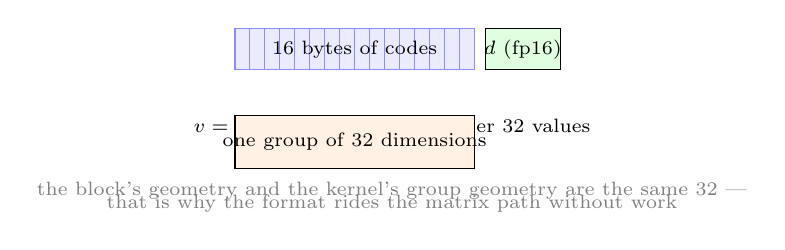
\begin{tikzpicture}[scale=0.95, every node/.style={font=\scriptsize}]
  % one block: 32 values along head_dim, 16 byte codes, one fp16 step
  \draw[fill=blue!8] (0,0) rectangle (3.2,0.55);
  \foreach \i in {0,...,15} {
    \draw[blue!45] ({0.2*\i},0) rectangle ({0.2*\i+0.2},0.55);
  }
  \node at (1.6,0.27) {16 bytes of codes};
  \draw[fill=green!12] (3.35,0) rectangle (4.35,0.55);
  \node at (3.85,0.27) {$d$ (fp16)};
  \node[align=center] at (2.1,-0.78) {$v=(\text{code}-8)\cdot d$, one step per 32 values};
  % the kernel's geometry underneath
  \draw[fill=orange!10] (0,-1.32) rectangle (3.2,-0.62);
  \node at (1.6,-0.97) {one group of 32 dimensions};
  \node[align=center,gray] at (2.1,-1.62) {the block's geometry and the kernel's group geometry are the same 32 ---};
  \node[align=center,gray] at (2.1,-1.80) {that is why the format rides the matrix path without work};
\end{tikzpicture}
\caption{The block and the kernel's group: 32 values along the head dimension carry one step, and the
prompt attention applies the step per group of 32 dimensions. The two geometries coincide, so the format's
reconstruction is exactly the map the kernel performs.}
\label{fig:block}
\end{figure}


\section{The Implementation}
\label{sec:impl}

\subsection{Reading the pool in the prompt kernel}

The batched prompt attention gained a 4-bit instantiation: the operand build produces the block's codes
and its step instead of 8-bit codes and a scale, the accumulator applies the step per group as before, and
the value path reads the codes of the same block geometry. In the parity harness the 4-bit arm runs against
an FP64 reference and against the old kernel, and its cost in the first version of the kernel was a
\textbf{5.12 times} shorter prompt read (97.3 to 19.0\,ms per chunk, same harness, same selection).

\subsection{The window pass}

The sibling paper's format keeps the most recent $S{=}256$ cells and the first $R{=}64$ sink cells of each
cache-carrying layer exact, in fp16, in a resident side pool; the rest is 4-bit\,\cite{kvwin}. That window
has to be read by the same kernel, and the two paths (quantized and exact) had to be merged: a window cell
stores nothing quantized, its value comes from the side pool, and the mask that decides which is which is
per lane. The implementation adds a second value set and a window-row lookup per cell, and it adds the
exact cells as a second operand for the affected positions.

\subsection{The parity harness}

The harness (\texttt{hip\_prompt\_attn\_wmma}) runs the prompt attention against an FP64 reference and
against the old kernel over a set of shapes, and it is the gate: a shape that fails stops the release. Its
output is a checksum per shape, and the checksums of the unchanged shapes are bit-identical across the
4-bit work --- the 4-bit path did not move a single bit of the 8-bit path.

\subsection{The occupancy lesson}
\label{sec:occupancy}

One implementation detail is worth its own paragraph, because it is not about the format. The second value
set (the window's exact cells) was first added to the 8-bit instantiation as well, as a 32-register
accumulator written only under a runtime condition. The 8-bit prompt kernel fell from 8.07 to \textbf{17.4\,ms
per chunk} (factor 2.16) --- with a bit-identical output. Guarding the whole window mechanism with
\texttt{if constexpr} (and taking \texttt{Q4 ? tmpw : 0} in the accumulation) brought it back to 8.26\,ms.
The lesson is general and it is the reason this paper reports kernel times next to every format change: on
this kernel the occupancy, not the arithmetic, decides by a factor of two.

\section{The Measurements}
\label{sec:meas}

All measurements are on one machine: a Windows PC with an RDNA4 card (gfx1201), ROCm 7.2, the engine built
from this tree (version \texttt{0.1.63-q4u32}), the model Swift-Qwen3.8-Flash-Next-GSQ-RCO-IQ3\_XXS,
the corpus the needle test (three depths, 30.782--30.783 prompt tokens at a 32K context). The prompt rate is
the median over the three requests of a run; the runs that appear in a table are named, and the series is
documented run by run in the in-repo record\,\cite{fastpath}. Where a comparison runs in two different
\emph{levels} (the machine has two throughput levels, and a run's level is not predictable from outside),
the comparison is made inside one level and the level is stated.

\begin{table}[t]
\centering
\caption{The measurements of the product path (all on the machine named above; the rates are medians over
the three requests of a run, the parity is the harness's worst deviation against an FP64 reference on a scale
of $\approx 7.5$).}
\label{tab:meas}
\begin{tabularx}{\linewidth}{@{}lXX@{}}
\toprule
Series & What it measures & Result \\
\midrule
A.~17 (parity) & the 4-bit arm against FP64 & green, $5.7$--$8.3\cdot10^{-6}$ \\
A.~18 (route) & the engine's own route line & matrix core in every run \\
A.~21 (price) & the format without the path & 264.3 tok/s ($2.5\times$ slower) \\
A.~22 (coupling) & the format with the path & $-1.8\%$ mean, $-2.1\%$ median \\
A.~23 (default) & the engine without \texttt{-{}-kv} & \texttt{q4u32} in 3 of 3 runs \\
A.~23 (slots) & the freed memory & $+18.7\%$ expert slots \\
\bottomrule
\end{tabularx}
\end{table}

\subsection{The parity}

The harness is green: the worst deviation of the 4-bit arm against the FP64 reference is
$5.7\cdot10^{-6}$ to $8.3\cdot10^{-6}$ on a scale of $\approx 7.5$, the same order as the decode kernel
itself ($4.7$ to $7.2\cdot10^{-6}$), and the shapes that do not use the window are bit-identical to their
previous checksums. The harness is also the cheapest possible evidence in this paper: it runs on the
machine in minutes and needs no model.

\subsection{The route, in the engine's own words}

The engine prints a line at start-up that names the format it chose and the route it takes. In the
series of runs that measures the default, that line reads \texttt{KV storage: q4u32 (the default on this
part: 54.5\,\% of int8's bytes, level with it at 32K; \dots)} in three of three runs, and the matrix-core
route line appears in each of them. The needle run finds 18 of 18 needles in the six runs of the series.
That is a route check, not a speed comparison, and it is reported as such.

\subsection{The speed, and the level}

The rates of the machine fall into two levels, and a run's level is not predictable from outside (the fast
level is not a measurement of anything the series controls; it appeared in one of twelve \texttt{int8}
requests in an earlier series and in three of six in another). The comparisons below are therefore made
inside one level and the level is named.

In the slow level the 4-bit format with the matrix path sits at \textbf{651.6} tokens per second against
\textbf{663.6} for \texttt{int8} over nine and six requests respectively: $-1.8\%$ on the mean, $-2.1\%$ on
the median, with the per-request spread of both arms overlapping (636.0--682.5 against 641.3--664.8). The
pre-registered criterion was ``not more than 5\% behind'', and the harness's own noise floor is 2--3\%; the
result is inside both. The same series measured the format without the path at 264.3 tokens per second
($-60.2\%$), which is the price of Section~\ref{sec:problem} and the reason the path is a precondition of
the format rather than an optimization of it.

\subsection{The memory, and what it buys}

The freed bytes are not an end in themselves; the engine spends them on the expert cache. With
\texttt{-{}-expert-cache auto} the 4-bit format holds \textbf{3428.7} expert slots on average (3438, 3414,
3434 in three runs) against \textbf{2888.5} for \texttt{int8} (2917, 2860 in two runs): \textbf{$+18.7\%$}
more resident experts, at a prompt rate that is $0.7\%$ behind (median $0.1\%$). This is the trade the
format exists for, and it is measured on the same machine in the same series.

\subsection{The default}

Without \texttt{-{}-kv} the engine of this tree chooses \texttt{q4u32} on gfx12 and 16-bit everywhere else,
and says which in its start-up line. The choice is the card's, because the card's prompt path is what
decides whether the format can be served: on a part without the matrix path the same format is 2.5 times
slower, and a format that costs 60\% of the prompt rate must not be the default there.

\section{The Ablation: what the format needs}
\label{sec:ablation}

The ablation is run on the engine's own cells: 768 records, 392.952 tokens, 201.191.424 values per side,
12 cache-carrying layers, the same dump the sibling campaign used\,\cite{shear}. The metric is the mean
squared error per value, in dB against the format itself. The parts, from the sibling campaign's
measurements and from this paper's:

\begin{table}[t]
\centering
\caption{What the format needs (block error in dB; the first three rows are the sibling campaign's
measurements on the same blocks\,\cite{shear}, the last two are this paper's).}
\label{tab:ablation}
\begin{tabularx}{\linewidth}{@{}lXX@{}}
\toprule
Part & Price & What it means \\
\midrule
fitted step (vs.\ block maximum) & $0.43$\,dB & the step is fitted, not from the maximum \\
codebook (Lloyd vs.\ uniform grid) & $0.43$\,dB & the codebook barely matters \\
power-of-two step (vs.\ fitted) & $1.81$\,dB & a UE8M0 exponent is expensive here \\
per-block zero point & $0.86$\,dB & buys range, costs $0.5$ bit per cell \\
per-coordinate scale (A.~26) & $+1.26$\,dB & \textbf{worse}: the channel axis is closed \\
group size 64 (A.~27) & $+0.92$\,dB & saves 0.25 bit per value; the kernel can serve it \\
group size 16 (A.~27) & $-1.19$\,dB & wins, but costs 0.5 bit per value and is not buildable \\
\bottomrule
\end{tabularx}
\end{table}

\subsection{The scale is the load-bearing part}

Three of the four rows say the same thing from different directions: the \emph{per-block scale} carries the
quality and the \emph{codebook} barely matters. A fitted Lloyd table on the same blocks costs 0.43\,dB
against the uniform grid; a second least-squares pass after the code assignment --- the only free change
left in the writer --- is worth 0.079\,dB, a twentieth of the 4K resolution\,\cite{shear}. This is the
finding UltraQuant reports for its own format (``with the per-block scale in place the codebook itself
barely matters'')\,\cite{ultraquant}, measured here on this engine's blocks: the same conclusion on
different hardware and a different corpus. It is also why the format is what it is: a uniform grid with a
fitted step is the cheapest to write, the cheapest to read, and the one the kernel's hardcoded value
mapping accepts.

\subsection{The channel axis is closed}
\label{sec:channel}

The 4-bit literature's advice for the sub-8-bit regime is asymmetric grouping: the key side per channel,
the value side per token, because a few outlier channels would otherwise poison their neighbours in a
group\,\cite{kivi}. The sibling campaign killed half of that axis before this paper existed: the S2 probe
found that the pre-rotation channels are not the heavier tail (mean excess kurtosis $-0.18$ before against
$-0.14$ after), so a per-channel \emph{scale} was not built\,\cite{shear}. What was open was the same axis
\emph{after} the rotation --- the axis the format actually sees --- and A.~26 closes it with a measurement
on the same blocks.

The arms: the format itself (one step per 32 values along the head dimension, per token), the same
quantizer with one step per coordinate over all tokens (the per-channel arm), and the hybrid of both
(K per coordinate, V per token, which is the literature's recipe). The result is the opposite of a gain:
the per-coordinate scale is \textbf{1.26\,dB worse} on the key side (768 records, 392.952 tokens, 201.191.424
values per side --- 6.29 million blocks; the MSE rises from $1.4937\cdot10^{-2}$ to
$1.9970\cdot10^{-2}$) and 0.40\,dB worse on the value side, and it is worse on the key side in
\textbf{12 of 12 layers} ($+0.72$ to $+1.65$\,dB). The hybrid inherits the key-side loss unchanged.

The reason is visible in the same run. The question of which coordinates set the scale in the format
itself has an answer: the five strongest of 256 coordinates set only \textbf{6.3\,\% to 13.6\,\%} of the
blocks, layer by layer. There are no outlier coordinates. After the rotation the dynamic range lives in
the \emph{token} --- every row has its own scale --- and the format's geometry follows that. A scale per
coordinate must cover the extreme token of that coordinate and is therefore too coarse for the typical
one.

Two consequences. First, the literature's warning does not survive the rotation: it holds for a format
without one. Second, the surviving part of the channel axis is the \emph{offset}, not the scale: removing a
fixed per-channel offset before the rotation is worth 1.70\,dB on the key side and 4.63\,dB on the value
side\,\cite{shear}, and it is a per-model table of 48\,KB. The scale axis is closed twice, once before and
once after the rotation, and each closure is a measurement.

\subsection{What stays open}

The group size of the block is the one knob the sibling campaign never varied, and A.~27 varies it here on
the same blocks: a group of 16 wins 1.19\,dB and costs 0.5 bit per value more (5.0 against 4.5), a group of
64 loses 0.92\,dB and saves 0.25 bit per value (4.25 against 4.5).

The kernel decides which of the two is buildable, and the rule is not the obvious one. The prompt attention
applies the step per group of 32 dimensions, and a block is a row along the head dimension --- so a block
that is \emph{larger} than the kernel's group is served by the same step twice: the step is constant inside
each 32-dimension group, and the kernel folds it into the operand as it does now
(\texttt{engine/src/kernels/cuda/qsa\_prompt\_attn.cu}: the step of the group is read from the block, and the fold
multiplies the group's codes by it). A 64-value block would therefore need three local changes --- the block
index, the lane's offset inside the block, and the nibble rule, which goes from two quadrants to four --- and
the step lookup would read every second group's step from the same block. A block that is \emph{smaller}
than the kernel's group cannot be served at all: two blocks would fall inside one group, and the kernel
applies one step per group.

So the 32-value group is not the only buildable one, and the honest statement is a trade rather than a
closure: the 64-value group is buildable and saves 0.25 bit per value (5.6\,\% of the bulk, which on the
measured card is about 40 more resident experts, or 1.2\,\%), and it costs 0.92\,dB of block error --- about
0.0012 nats through the measured block-to-nats bridge\,\cite{shear}. Against a product arm that is already
level with \texttt{int8} on the mean and behind it on the p99, that is the wrong direction: it buys bytes by
spending the margin the format was chosen for. The 16-value group is the better codec and the more
expensive one, and it is not buildable. The group size therefore stays at 32 in the product, and the format
is fixed: \textbf{4.5 bit per cell, one step per 32 values, a uniform grid, no codebook, no zero point, no
calibration}. What is left open is not a format question: the per-channel offset (a property of the cache,
not a lever on this format), the RDNA3 and APU arms (Section~\ref{sec:limits}), and the integer path
(a kernel question, not a format one).

\paragraph{The one remaining format question is the byte model's.} The group's step costs half a bit per
value at 32 values and a quarter at 64; the quality side of that trade is now measured, and it says the
32-value group is the only one the kernel can serve (Section~\ref{sec:ablation}).

\section{The Product Path}
\label{sec:product}

\subsection{The engine chooses}

The engine of this tree is \texttt{0.1.63-q4u32}: the Strata release it was changed from, plus the
suffix of what it adds. Without \texttt{-{}-kv} it takes the format where the prompt path can serve it
(gfx12, and the parts whose matrix path is on) and 16-bit everywhere else; a format the person names is
always written, and \texttt{STRATA\_HIP\_WMMA=0} keeps 16-bit everywhere, because that is the state
without the prompt path, in which the format is 2.5 times slower. The engine's own line names the choice
at start-up.

\subsection{The Terminal follows}

A run config must not contradict the engine. The Terminal writes the format itself only where the engine
cannot choose: on every card that is not gfx12, on every engine that is not a \texttt{q4u32} build, and
above 8K context, where the last release named 8-bit anyway. Everywhere else it writes nothing and lets
the engine decide. The gate is the engine's \emph{variant}, not a version number --- the manifest carries
the variant, and the Terminal reads it --- so an upstream engine, which has no such default, keeps the
last release's behaviour exactly.

\subsection{An update never switches the variant}

A fork's engine and an upstream engine carry the same release number and differ in what they do, so a
version comparison cannot keep them apart. The package therefore carries the variant in its manifest, and
the update rule is the same one the CUDA build already follows (an update never switches the CUDA build):
a newer build of the \emph{same} variant is taken, a package of another variant is not offered, and the
update says so in one line. A \texttt{q4u32} engine cannot be replaced by an upstream engine by an update
that only meant to bring a newer version of the same thing.

\section{Limits and Open Questions}
\label{sec:limits}

\paragraph{The RDNA3 family (gfx11) and the integrated APUs.} The matrix-core prompt kernel of this engine
is written per architecture and \emph{has} an RDNA3 variant: its own intrinsic, its own fragment layout
(\texttt{PA\_KL} 16 instead of 8, a different accumulator row mapping), and the 4-bit path's nibble
expansion is consistent with it (statically: a 16-dimension step always falls inside one 32-value block).
With \texttt{STRATA\_HIP\_WMMA=1} the 4-bit pool runs on RDNA3 today; on the integrated parts (gfx1103,
gfx1151) that switch is even the default, and the prompt rate there was measured by the community
(4K 690 to 1.090 tokens per second on a Strix Halo box). What is missing is the \emph{default}: the
engine's format choice names gfx12, the Terminal follows it, and both are preregistered for RDNA3
(A.~24) and for the APUs (A.~25) with their criteria --- parity, the rate against \texttt{int8}, the
logit gate (the KL against the FP32 kernel and the top-p agreement) and the expert slots, separately for
the case with and without the KV streaming that the APUs use above 64K. The hardware is not on this
machine, so those arms are open and everything said about them here is static analysis or citation.

\paragraph{CUDA.} The engine's format choice is an AMD decision: on CUDA the 4-bit path is not built and
not measured on this branch, so the format choice stays 16-bit there and the Terminal names 8-bit, exactly
as before.

\paragraph{The bytes.} 4.5 bit per cell is the format's price, and half of it is the group's step. The
group size is the open knob (Section~\ref{sec:ablation}).

\paragraph{The offset.} The per-channel offset is worth decibels and costs 48\,KB per model and a basis
discipline\,\cite{shear}; it is not part of this format and was not measured together with it.

\section{Relation to Prior Work}

\paragraph{UltraQuant} is the closest published format to this cache: 4-bit codes with one scale per 32
values --- the same group size --- for long-context serving, on CDNA4\,\cite{ultraquant}. Two things carry
over. Its ablation --- the per-block scale carries the quality, the codebook barely matters --- is measured
here on this engine's blocks and comes out the same way (0.43\,dB for the codebook), on different hardware
and a different corpus. Its scale mechanism does not carry over: the UE8M0 exponent costs 1.81\,dB here
in its best form and 2.43\,dB in the paper's form, and on this hardware the exponent would save one byte
per block, so the trade would be voluntary here and forced there\,\cite{shear}. What this paper adds is the
other half of the format question: not what the scale costs, but that a 4-bit pool can be read by the
matrix core at all, and what that buys (a 2.5 times faster prompt path, and $18.7\%$ more resident
experts).

\paragraph{KIVI and the sub-8-bit literature} propose asymmetric grouping --- the key side per channel, the
value side per token\,\cite{kivi}, and a recent analysis of the sub-8-bit regime warns that the quality
breaks down below 8 bit and names the same axis\,\cite{zinc}. This paper measures that advice on this
format's own blocks and finds it does not transfer: a scale per coordinate is 1.26\,dB \emph{worse} on the
key side, in 12 of 12 layers, because the rotation has moved the dynamic range into the token
(Section~\ref{sec:channel}). The advice holds for a format without a rotation; ours has one, and the
measurement says which axis is alive.

\paragraph{The upstream 4-bit KV work in the LLM stack} dequantizes rather than reads: llama.cpp fuses the
dequantization into the MMA flash-attention kernels, so the prompt path no longer writes an fp16 scratch,
but the codes are still read as 8-bit or dequantized in registers\,\cite{llamacpp-pr}. A community fork
goes further and reads the 4-bit codes natively in the tensor-core path, with the query quantized to
8-bit\,\cite{torad}. SageAttention's RDNA4 backend puts the int8 query-key product and the fp8
value-product on the matrix cores\,\cite{sage}. None of them reads a 4-bit \emph{cache} directly into the
matrix core: the codes are dequantized on the way. The gap this paper closes is that one.

\paragraph{What the RDNA3 family has, and what it has measured.} The older family has matrix cores too:
AMD's documentation names the dense WMMA built-ins for gfx1100--gfx1103 and gfx1150--gfx1153, with the
same wave32 shape and the same 4-bit type at half the cycles of the fp16 type\,\cite{amdwmg,amdcalc}; the
matrix-multiply-accumulate type of the datacenter cards does not exist there\,\cite{amdcalc}, and the fp8
type does not either\,\cite{rocwmma}. AMD's own kernel work on RDNA3 (October 2026) reports a hand-written
WMMA GEMM ahead of the vendor library on a workstation card of that family (70.92 against 56.86
TFLOP/s\,\cite{amdbl}), which says that the family is worth writing kernels for. A community fork
measured a 34--75\,\% faster prompt on a 7900 XTX with a matrix-core prefill --- and the same run moved
the prefill logits measurably (KL 0.0293, top-p 92.59\,\% against the tile path)\,
\cite{stew}, which is why the preregistration of the RDNA3 arm in this line asks for a logit gate and not
only for a rate. A later community measurement of a natively read quantized KV cache on an integrated
RDNA3.5 part reports a decode gain of 3--6\,\%\,\cite{llamacpp-gfx1151}, against 1.4--1.9$\times$ on
RDNA4\,\cite{llamacpp-pr}: on the older family the bottleneck stays the memory bandwidth, and a 4-bit cache
promises memory there, not tempo.


\paragraph{The rotation} this format relies on belongs to the family that the quantization literature uses
to make outliers harmless\,\cite{quarot,rotatekv}, and the 2026 theory work shows that the sign-only
randomized Hadamard suffices\,\cite{rht-theory}. A systematic comparison finds the rotation worth nothing
where the data is isotropic and everything where it is heavy-tailed\,\cite{amd-kv-ablation}; the channel
moments measured on this model put it in the light-tailed regime, which is why the randomized variant is
not used here and why the channel axis has so little to offer (Section~\ref{sec:channel}).

\section{Threats to Validity}

\paragraph{One machine, one card.} Every measurement is a Windows PC with one RDNA4 card (gfx1201). The
level structure of the machine (Section~\ref{sec:meas}) is not understood; the comparisons are made inside
one level and the level is named, but a reader should treat the absolute rates as machine-specific and the
differences as the result.

\paragraph{One model, one corpus.} The route and the parity are properties of the kernel and are expected
to hold for any model of this shape; the rates are measured on one model with the needle corpus. The block
measurements use one corpus (cwe-4k) on the sibling campaign's dump.

\paragraph{The format is compared against \texttt{int8}, not against a better 4-bit format.} The claim is
that this format is served by the hardware at the level of \texttt{int8} and costs 54.5\,\% of its bytes. It is
not a claim that this format is the best 4-bit format; the sibling paper's campaign is the source for that
question\,\cite{shear}.

\paragraph{The pre-registration covers the comparisons, not every number.} The arms that are compared here
(A.~21, A.~22, A.~23, A.~26) were registered with their criteria before their first run; the block
measurements of the sibling campaign have their own registration\,\cite{shear}. Numbers that are neither
--- the per-layer breakdown, the level structure, the occupancy lesson --- are reported as what they are.

\paragraph{The hardware claims of the RDNA3 arm are static analysis.} The code paths exist and the
geometry is consistent; nothing in this paper measures them.

\section{Conclusion}

A 4-bit KV cache on RDNA4 was a memory win with a 2.5 times speed loss, because the matrix-core prompt
path could not read the pool. The format that removes the loss is not exotic: a uniform grid on blocks of
32 values with a fitted step, written after the rotation the cache already applies. Its property is that
it is affine along the head dimension, which is exactly the map the kernel applies per group of 32
dimensions, so it rides the fast path without a table, a codebook or a per-model artifact.

Measured on the machine named above: the parity harness is green ($5.7$--$8.3\cdot10^{-6}$ against FP64,
the 8-bit shapes bit-identical), the engine takes the matrix route in every run, the prompt rate is level
with \texttt{int8} ($-1.8\%$ mean, $-2.1\%$ median) at 54.5\,\% of its bytes, and the freed memory buys
\textbf{$+18.7\%$} expert slots. The ablation says what the format needs: the per-block scale is
load-bearing, the codebook is not (0.43\,dB), and the per-channel axis of the sub-8-bit literature is
closed by measurement (1.26\,dB worse, 12 of 12 layers). The product rule follows the measurement: the
card chooses the format where the path was measured, every other card and every upstream engine keeps the
last release's behaviour, and the variant is marked so that an update cannot silently replace it.

The open arms are the RDNA3 and APU extensions (pre-registered, no hardware here), the group size of the
block, and the CUDA path.

\begin{thebibliography}{9}

\bibitem{fastpath}
M.~Kronenberger.
\emph{The \texttt{q4u32} fast path: the run-by-run record} (working document, German).
In-repo, \texttt{bench/results/2026-11-14-q4u32-fastpath/}, 2026-11-17.
(The A.~16--A.~26 series; every table in this paper cites its entry.)

\bibitem{shear}
M.~Kronenberger.
\emph{Mean-Centered Calibrated KV Quantization: int8 Quality Below 5 bit/cell}.
In-repo, \texttt{docs/paper/}, version 0.24, 2026-11-14.
(The block measurements this paper inherits: the grid's geometry, the codebook's price, the
power-of-two step, the per-channel offset, the moments and the channel probe.)

\bibitem{kvwin}
M.~Kronenberger.
\emph{KV-Window-Hardening: the exact-cell window}.
In-repo, \texttt{docs/paper/}, version 1.11, 2026-11-11.
(The window the 4-bit path reads: 256 recent and 64 sink cells per layer, exact.)

\bibitem{ultraquant}
I.~Chakrabarti, D.~Limpus, A.~Ghai Rana, B.~Bao, S.~Tiwari, T.~Crepaldi, A.~Sirasao.
\emph{UltraQuant: 4-bit KV Caching for Context-Heavy Agents}.
EMNLP 2026 Industry Track, arXiv:2606.20474.

\bibitem{kivi}
Z.~Liu, J.~Yuan, H.~Jin, S.~Zhong, Z.~Xu, V.~Braverman, B.~Chen, X.~Hu.
\emph{KIVI: A Tuning-Free Asymmetric 2bit Quantization for KV Cache}.
ICML 2024, arXiv:2402.02750.

\bibitem{zinc}
\emph{Sub-8-Bit KV Cache Quantization Is Not a Free Lever for an RDNA4 Agent Swarm}.
zolotukhin.ai, 2026-08-14. (The KIVI-axis warning this paper measures on its own blocks.)

\bibitem{zincwmma}
\emph{int8 WMMA doubles RDNA4's matrix rate, and Q4\_K's block scales take half of it back}.
zolotukhin.ai, 2026-07-12. (The descaling asymmetry this paper's format avoids by keeping the scale on
the operand: 1.20$\times$ realized against a theoretical 2$\times$.)

\bibitem{amdwmg}
AMD.
\emph{ROCm Optimization Guide: RDNA4 dense WMMA built-ins} (rates, signatures, the lane-group split).
2026. (The rate table of Section~\ref{sec:kernel}.)

\bibitem{amdcalc}
AMD.
\emph{Matrix Instruction Calculator} (the \texttt{rdna3} block: the dense WMMA built-ins and their
execution cycles; no matrix-multiply-accumulate type on that family). 2026.

\bibitem{rocwmma}
AMD.
\emph{rocWMMA: data-type support} (the fp8 and BF8 types require gfx1200/gfx1201; the integer and fp16
types are available on gfx11) and \emph{installation} (the supported gfx11 targets). 2026.

\bibitem{amdbl}
A.~Johar, J.~Stephan, I.~Kiss.
\emph{FP16 GEMM Optimization on AMD RDNA 3 and RDNA 4 Architectures}.
AMD ROCm blog, 2026-10-16. (Measured: a hand-written WMMA kernel against the vendor library on a
workstation card of the RDNA3 family.)

\bibitem{stew}
\texttt{stew675/llama-cpp-rdna-boosts} PR \#199: matrix-core flash attention with head 512 on gfx1100.
2026-10-21. (Measured on a 7900 XTX: the prompt rate and the logit shift of that path.)

\bibitem{llamacpp-gfx1151}
\texttt{ggml-org/llama.cpp} PR \#31234, with the measurement of 2026-11-16 on an integrated RDNA3.5 part:
a natively read quantized KV cache in the tile path. 2026.


\bibitem{llamacpp-pr}
\texttt{ggml-org/llama.cpp} PR \#31802: fused \texttt{q4\_0} dequantization in the MMA
flash-attention kernels. 2026-11.

\bibitem{torad}
\texttt{torad-labs/llama.cpp}, commit \texttt{60feea0}: native \texttt{q4\_0} in the
tensor-core path, 8-bit query. 2026.

\bibitem{sage}
\texttt{thu-ml/SageAttention} PR \#368: native gfx12 backend (int8 query-key product,
fp8 value-product on the matrix cores). 2026.

\bibitem{quarot}
S.~Ashkboos, A.~Mohtashami, M.~L.~Croci, B.~Li, P.~Cameron, M.~Jaggi, D.~Alistarh, T.~Hoefler, J.~Hensman.
\emph{QuaRot: Outlier-Free 4-Bit Inference in Rotated LLMs}.
arXiv:2404.00456, 2024.

\bibitem{rotatekv}
Z.~Su, Z.~Chen, W.~Shen, H.~Wei, L.~Li, H.~Yu, K.~Yuan.
\emph{RotateKV: Accurate and Robust 2-Bit KV Cache Quantization for LLMs via Outlier-Aware Adaptive Rotations}.
arXiv:2501.16383, 2025.

\bibitem{quip}
A.~Tseng, J.~Chee, Q.~Sun, V.~Kuleshov, and C.~De~Sa.
\emph{QuIP\#: Even Better LLM Quantization with Hadamard Incoherence and Lattice Codebooks}.
ICML 2024, arXiv:2402.04396.

\bibitem{rht-theory}
R.~Ben-Basat, W.~Kuszmaul, M.~Mitzenmacher, A.~Portnoy, and S.~Vargaftik.
\emph{Quantizing With Randomized Hadamard Transforms: Efficient Heuristic Now Proven}.
arXiv:2605.06014, 2026.

\bibitem{amd-kv-ablation}
P.~D'Alberto, A.~Sirasao, E.~Delaye, and R.~Patwari.
\emph{Ablation, Statistical Inference, and Validation for KV-Cache Compression}.
arXiv:2607.09683, 2026.

\bibitem{optr}
\emph{Output-Aware Rotation for INT2 KV-Cache Quantization}.
arXiv:2608.02691, 2026.

\bibitem{offq}
\emph{OffQ: Taming Structured Outliers in LLM Quantization by Offsetting}.
arXiv:2606.07116, 2026.

\bibitem{great-inversion}
E.~Jokar.
\emph{Transforms for LLM Quantization: The Great Inversion and Format Co-Design}.
arXiv:2608.25188, 2026.

\bibitem{hadanorm}
G.~Federici et~al.
\emph{HadaNorm: Adaptive Channel Centering for Post-Hadamard Quantization}. 2025.

\bibitem{llamacpp-center}
\emph{KV-cache mean-centering and its calibration-basis guard}.
Public \texttt{llama.cpp} fork (PrismML-Eng), July 2026.

\bibitem{streamingllm}
G.~Xiao, Y.~Tian, B.~Chen, S.~Han, M.~Lewis.
\emph{Efficient Streaming Language Models with Attention Sinks}.
arXiv:2309.17453, 2023 (ICLR 2024).

\bibitem{ansatz}
M.~Kronenberger.
\emph{Ansatz-Verbesserungen: KV-Cache-Quantisierung \& Exact-Cell-Fenster}
(working document, German). In-repo, \texttt{docs/paper/}, 2026-10-25.

\end{thebibliography}

\end{document}
